\vskip1cm
\begin{table}[H]
	\centering
	\caption*{2班2组CAD画图分工表}
	% \resizebox{\textwidth}{!}{}
	\begin{tabular}{cccc}
		\toprule
		附图    & 图名    & 设计    & 学号 \\
		\midrule
		1     & 格栅及曝气沉砂池平剖面图 & 张晓满  & 202019020202 \\
		2     & 改良卡鲁塞尔氧化沟平剖面   & 赵梦雪  & 202019020201 \\
		3     & 二沉池平剖面图   & 吴恒    & 202019020229 \\
		4     & 加压溶气气浮池 & 梁政儒   & 202019020204 \\
		5     & 臭氧消毒池平剖面图   & 梁静    & 202019020203 \\
		6     & 提升泵房平剖面图  & 安德利   & 202019020220 \\
		\midrule
		7     & 污水处理厂平面布置图  & \multicolumn{2}{c}{2班2组} \\
		8     & 污水处理厂高程布置图  & \multicolumn{2}{c}{2班2组} \\
		\bottomrule
	\end{tabular}
\end{table}

\thumbnail{格栅及曝气沉砂池平剖面图}
\begin{figure}[H]
	\centering
	\rotatebox{90}{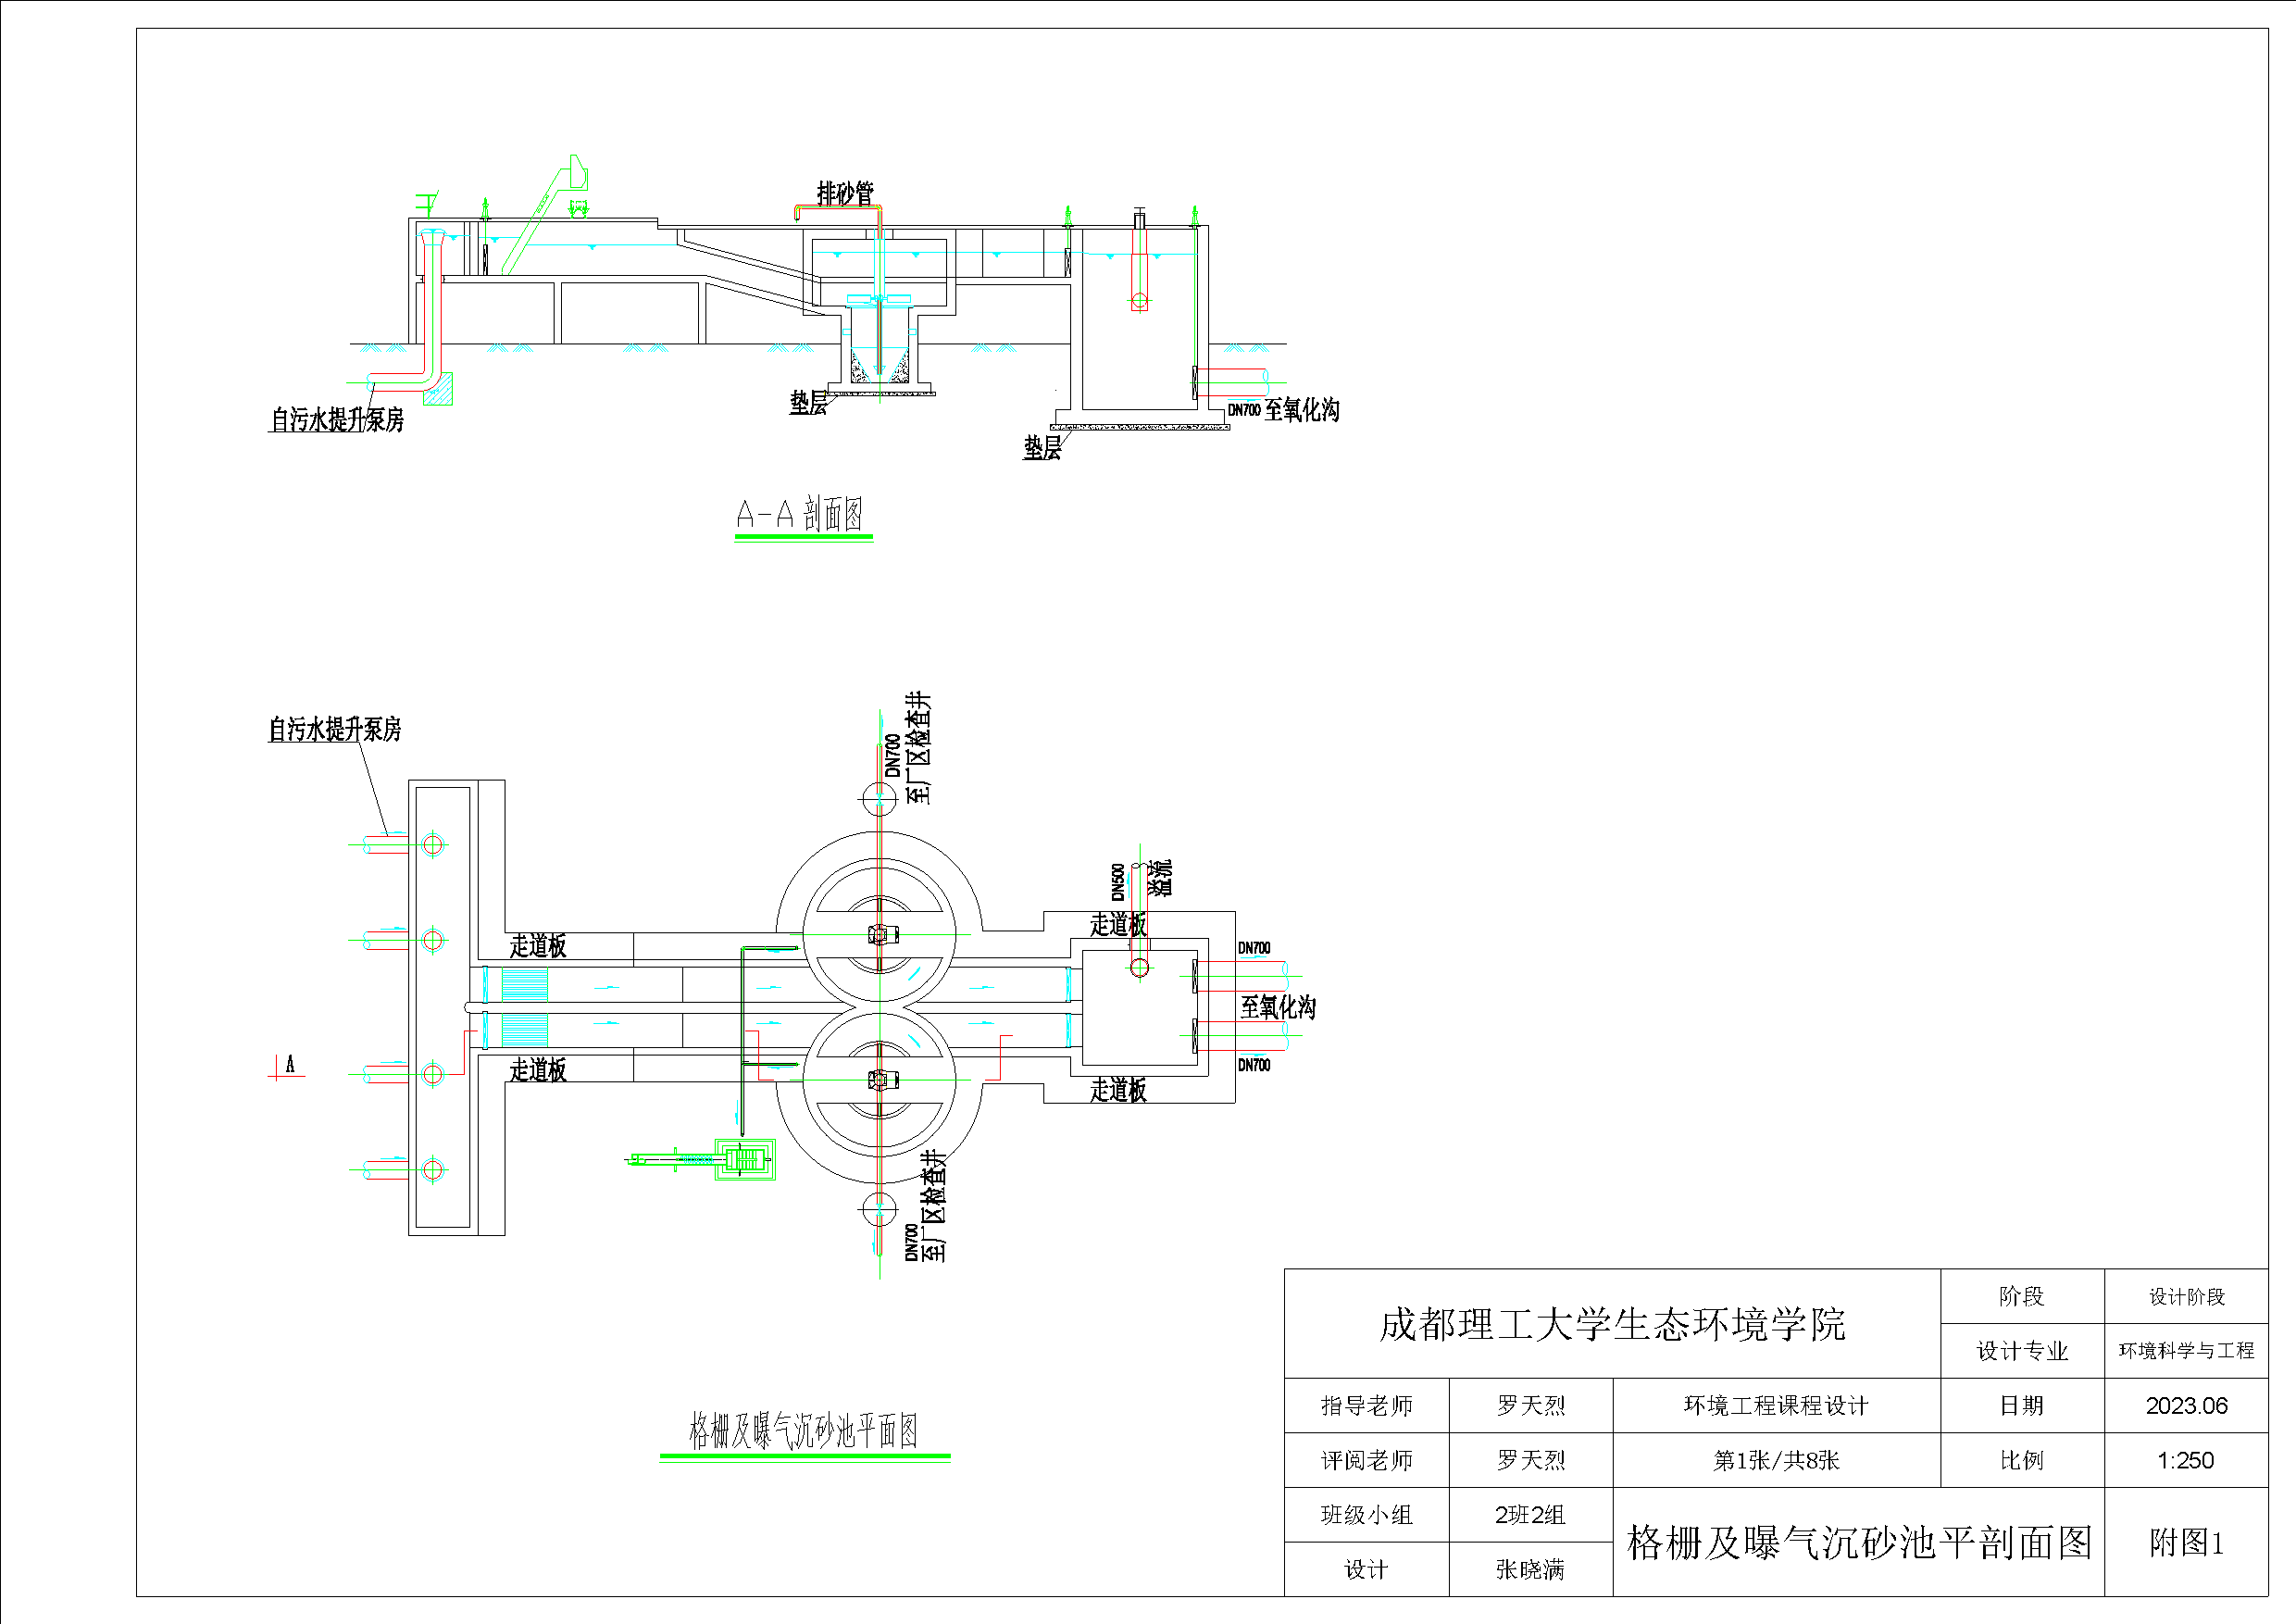
\includegraphics[width=1.15\textwidth]{drawing/Flat profile view of aeration grit tank.pdf}}
\end{figure}

\thumbnail{改良卡鲁塞尔氧化沟平剖面}
\begin{figure}[H]
	\centering
	\rotatebox{90}{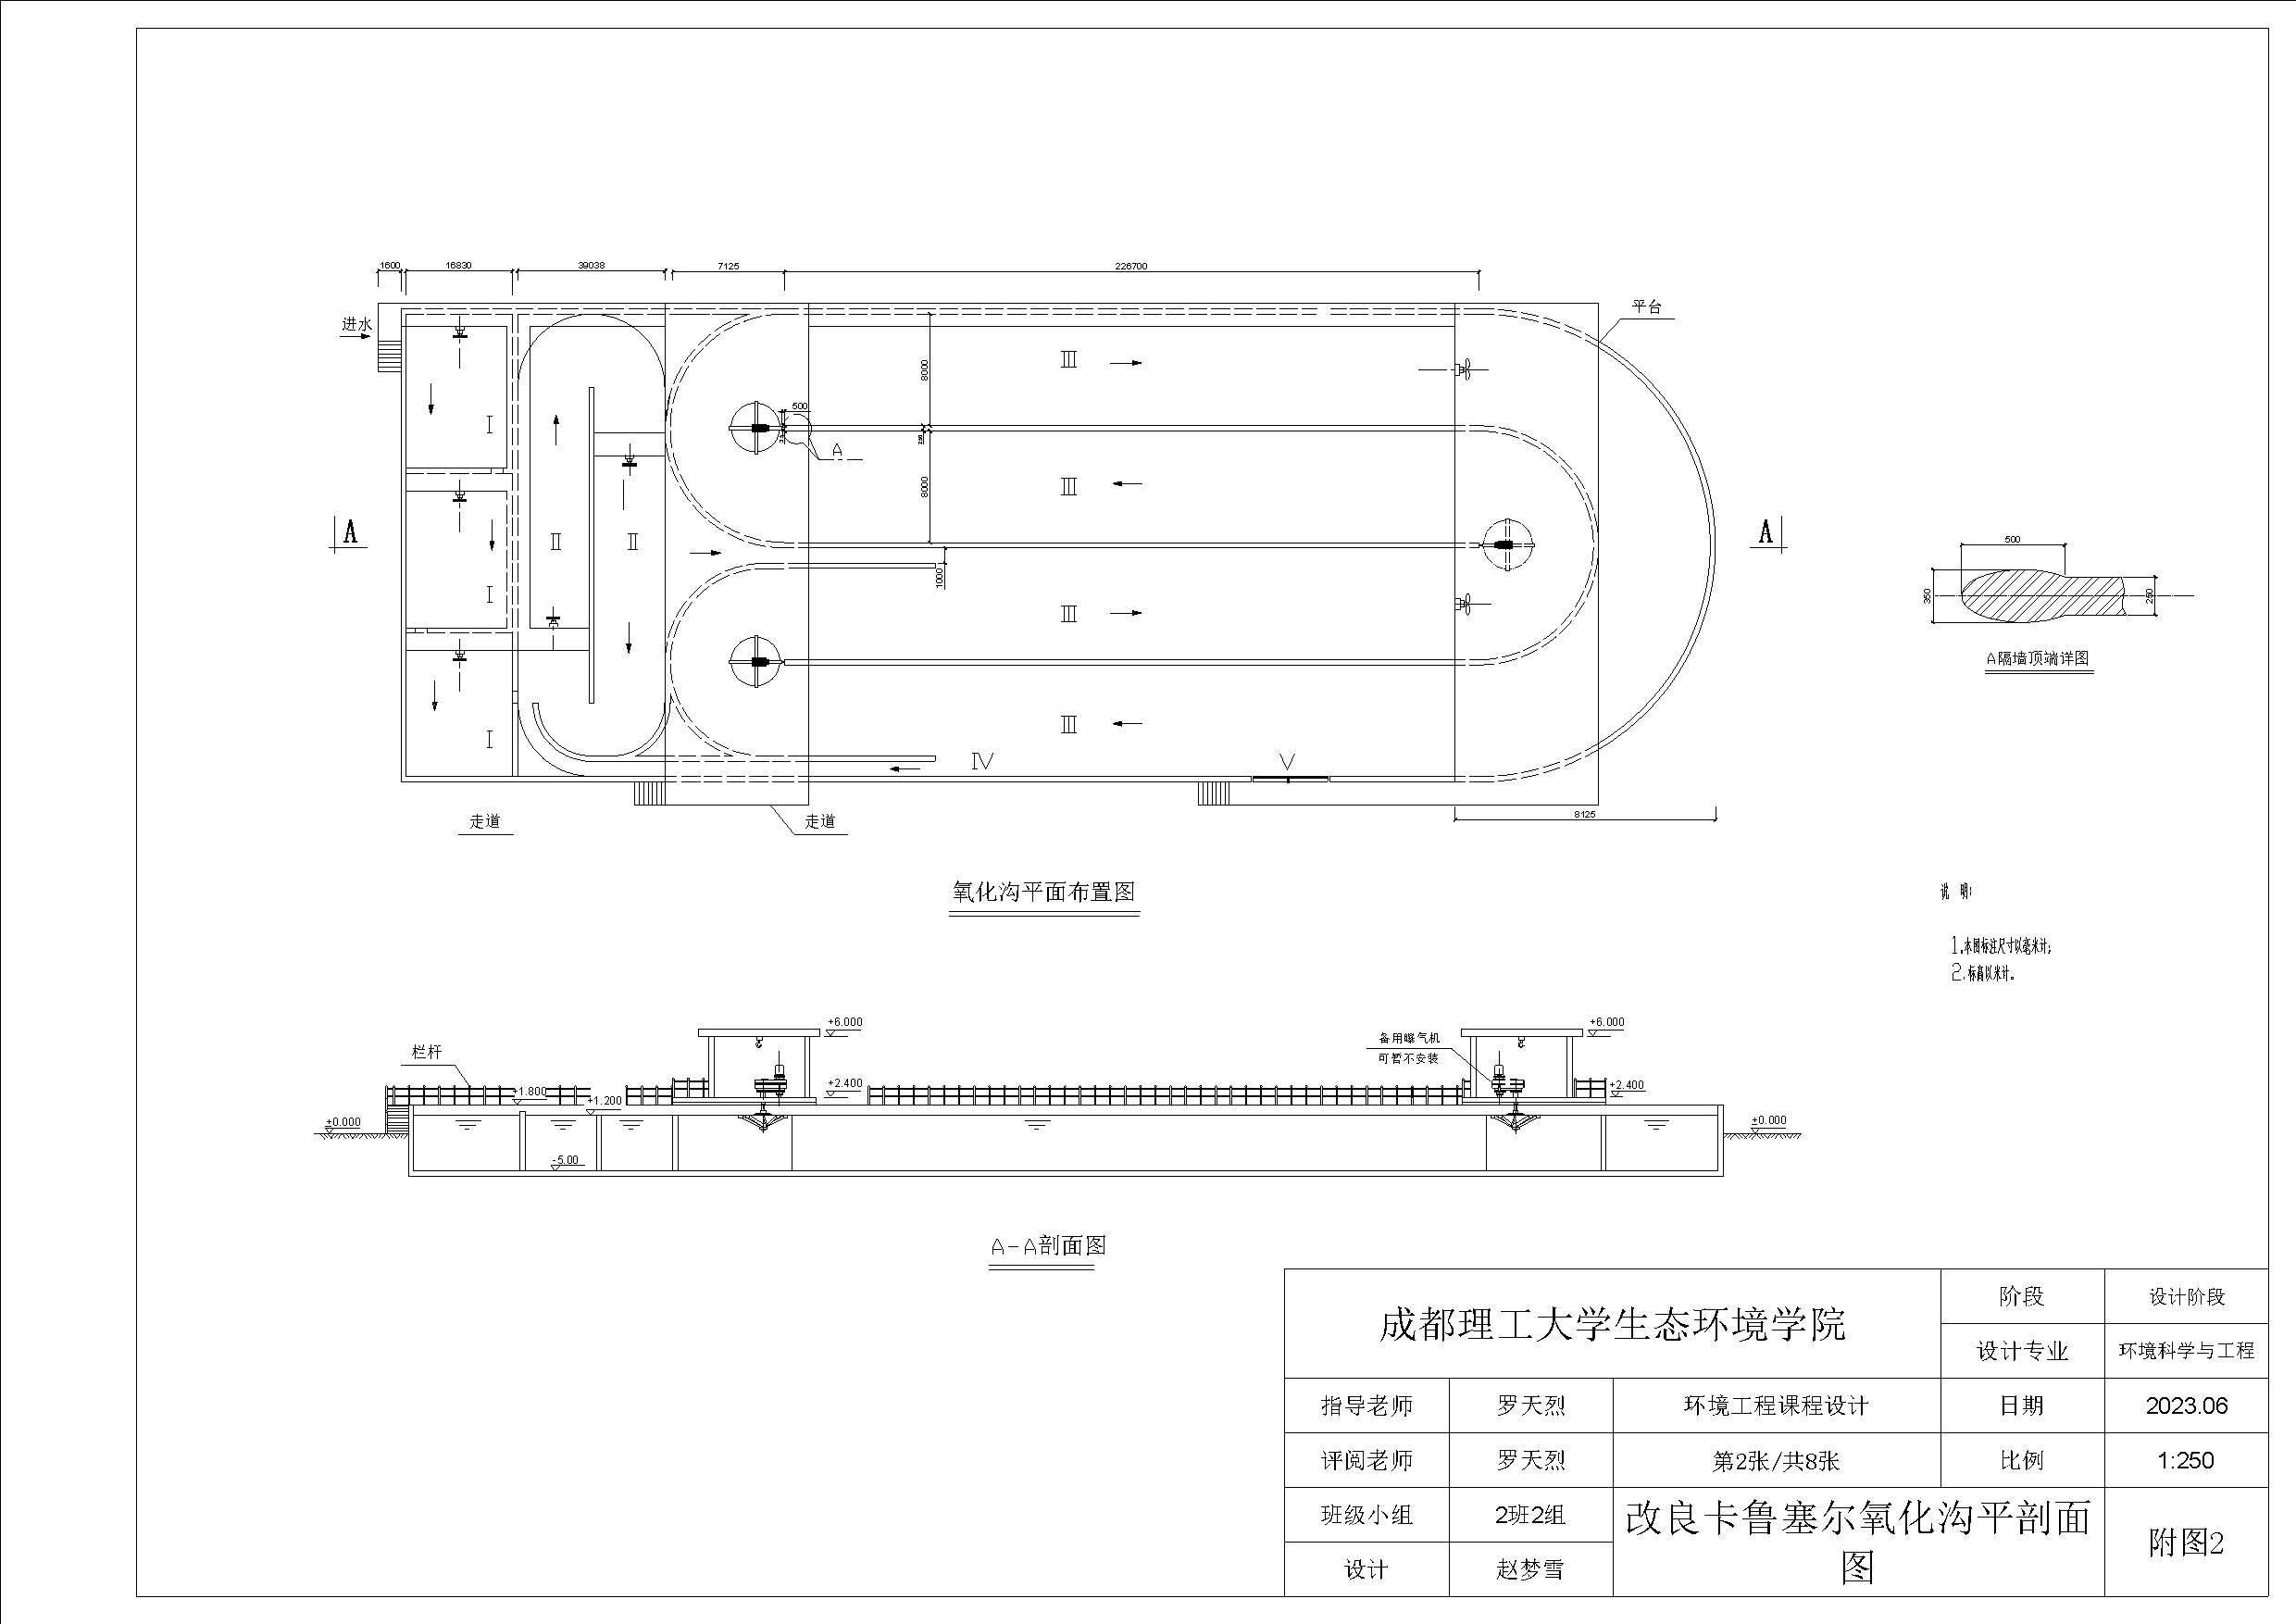
\includegraphics[width=1.15\textwidth]{drawing/Modified Carrousel oxidation groove flat profile.pdf}}
\end{figure}

\thumbnail{二沉池平剖面图}
\begin{figure}[H]
	\centering
	\rotatebox{90}{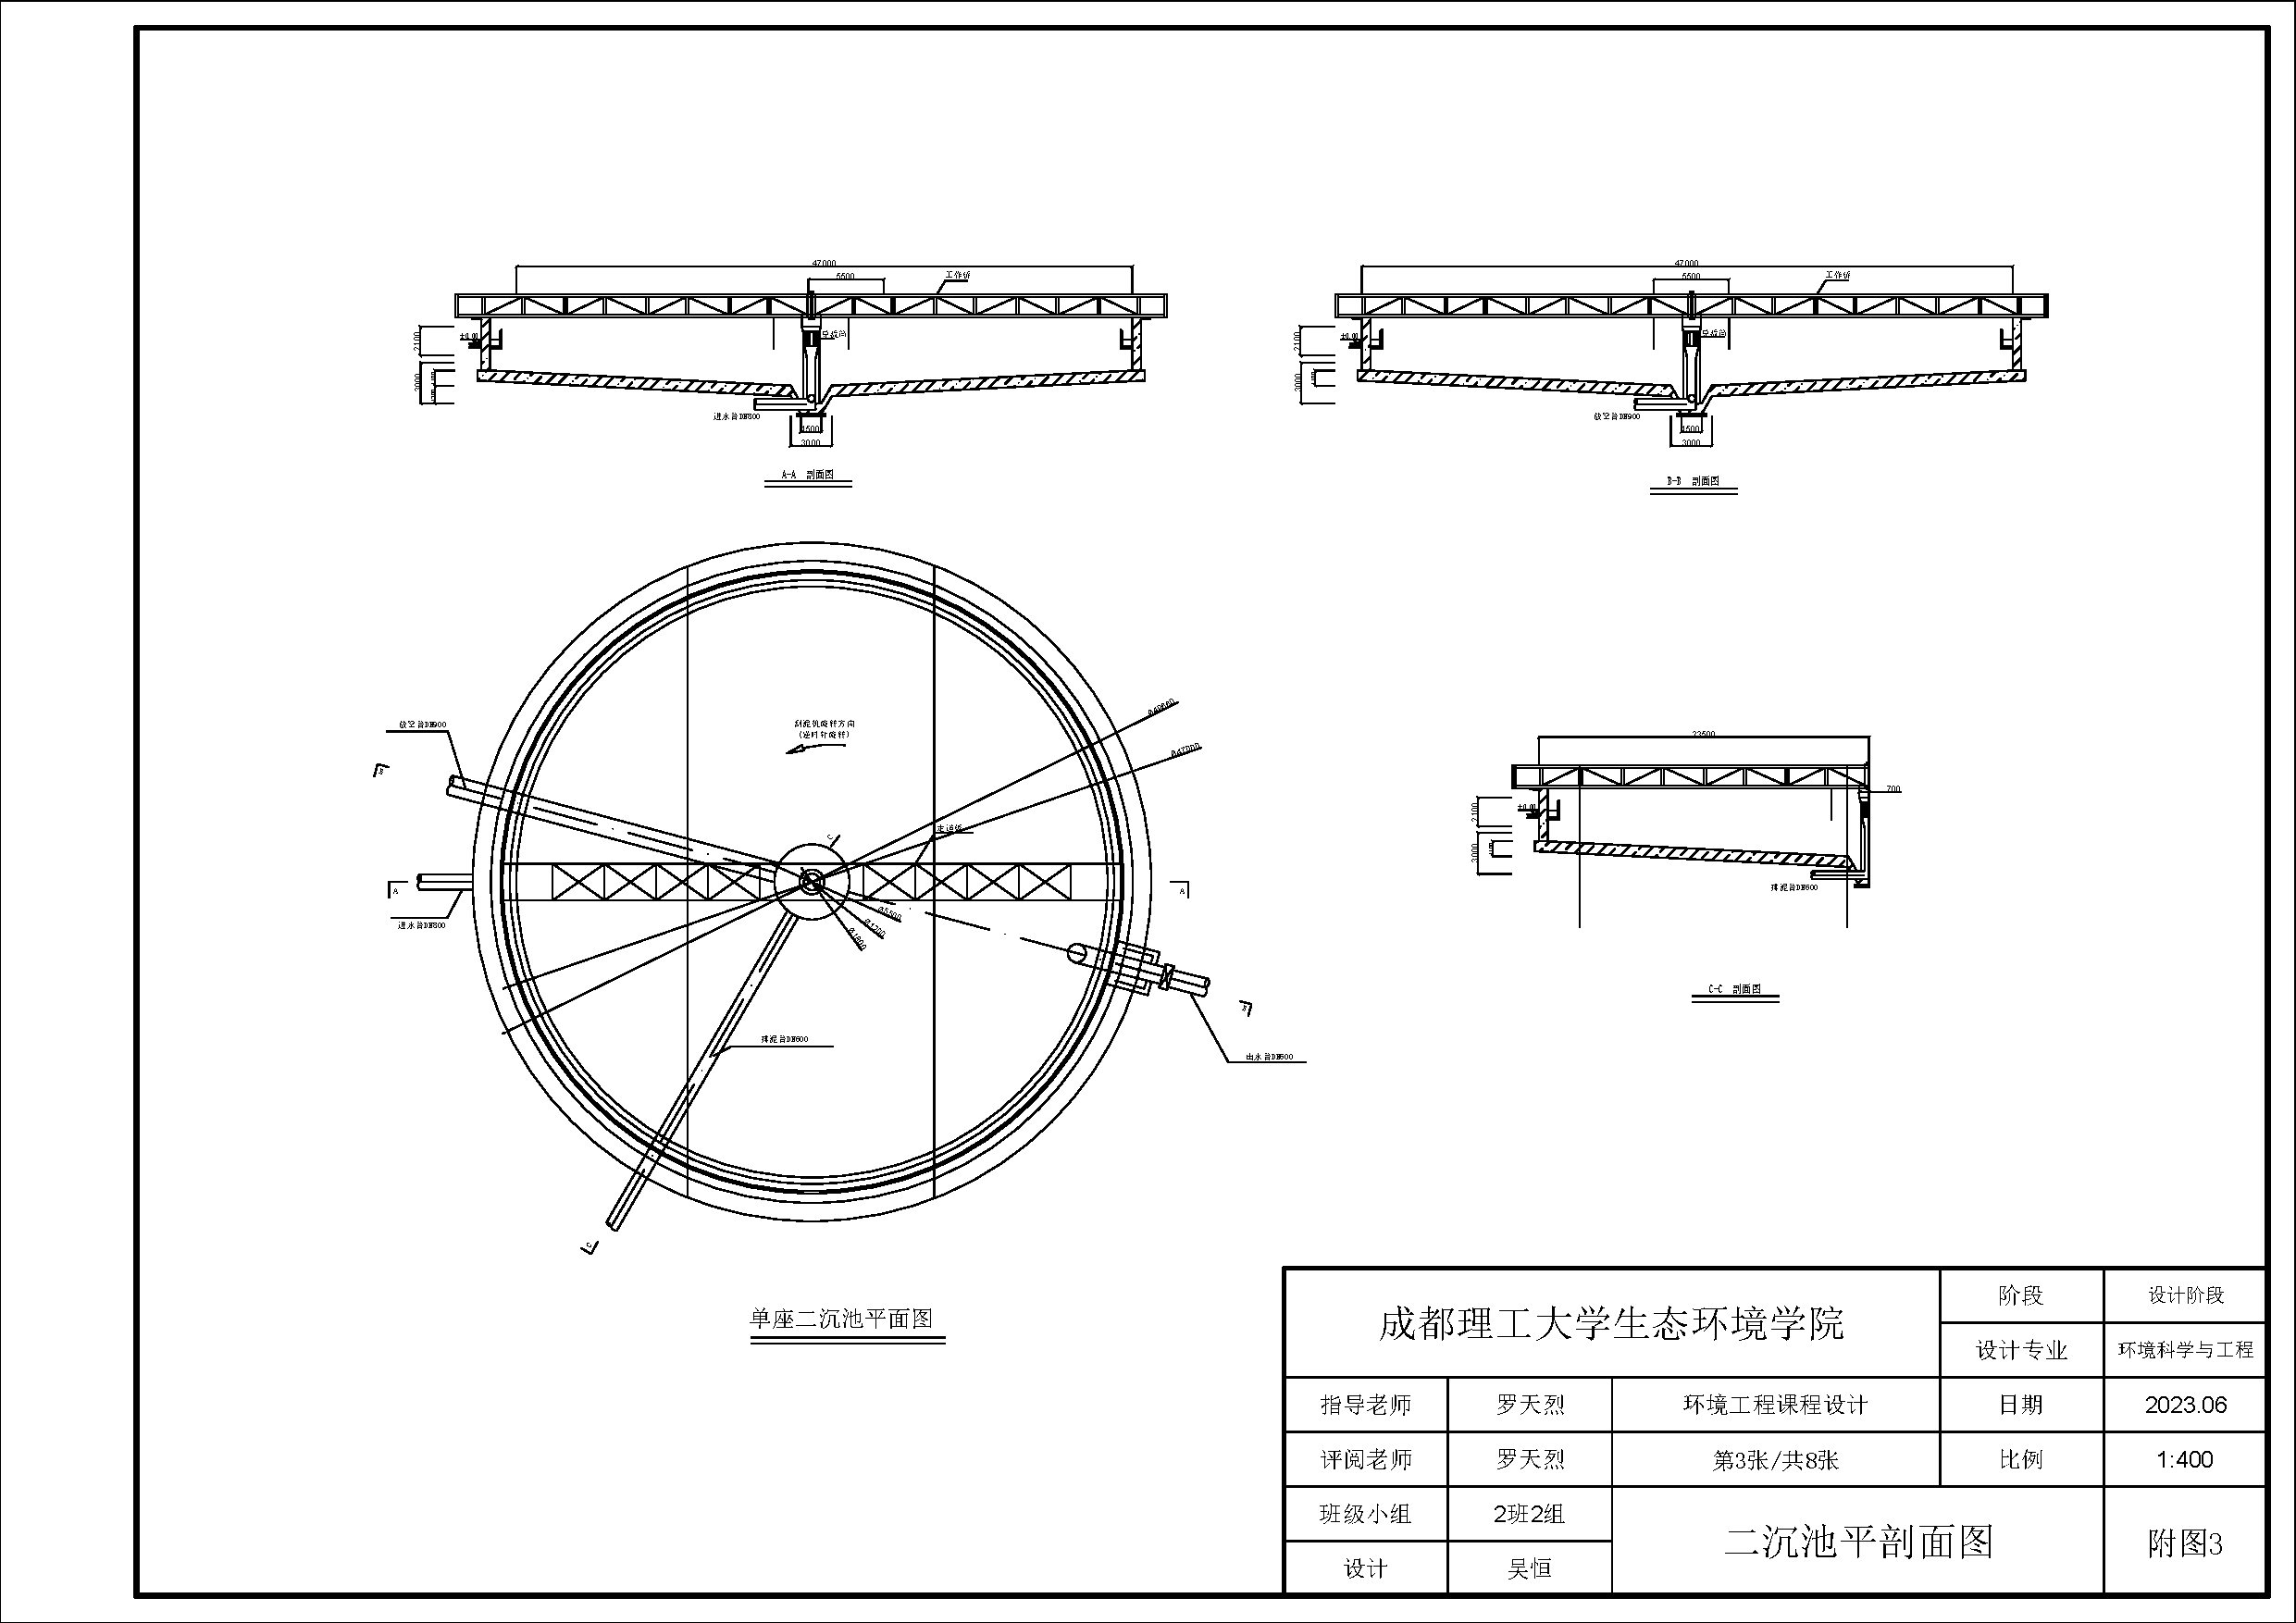
\includegraphics[width=1.15\textwidth]{drawing/2. Flat profile view of the sedimentation tank.pdf}}
\end{figure}

\thumbnail{加压溶气气浮池}
\begin{figure}[H]
	\centering
	\rotatebox{90}{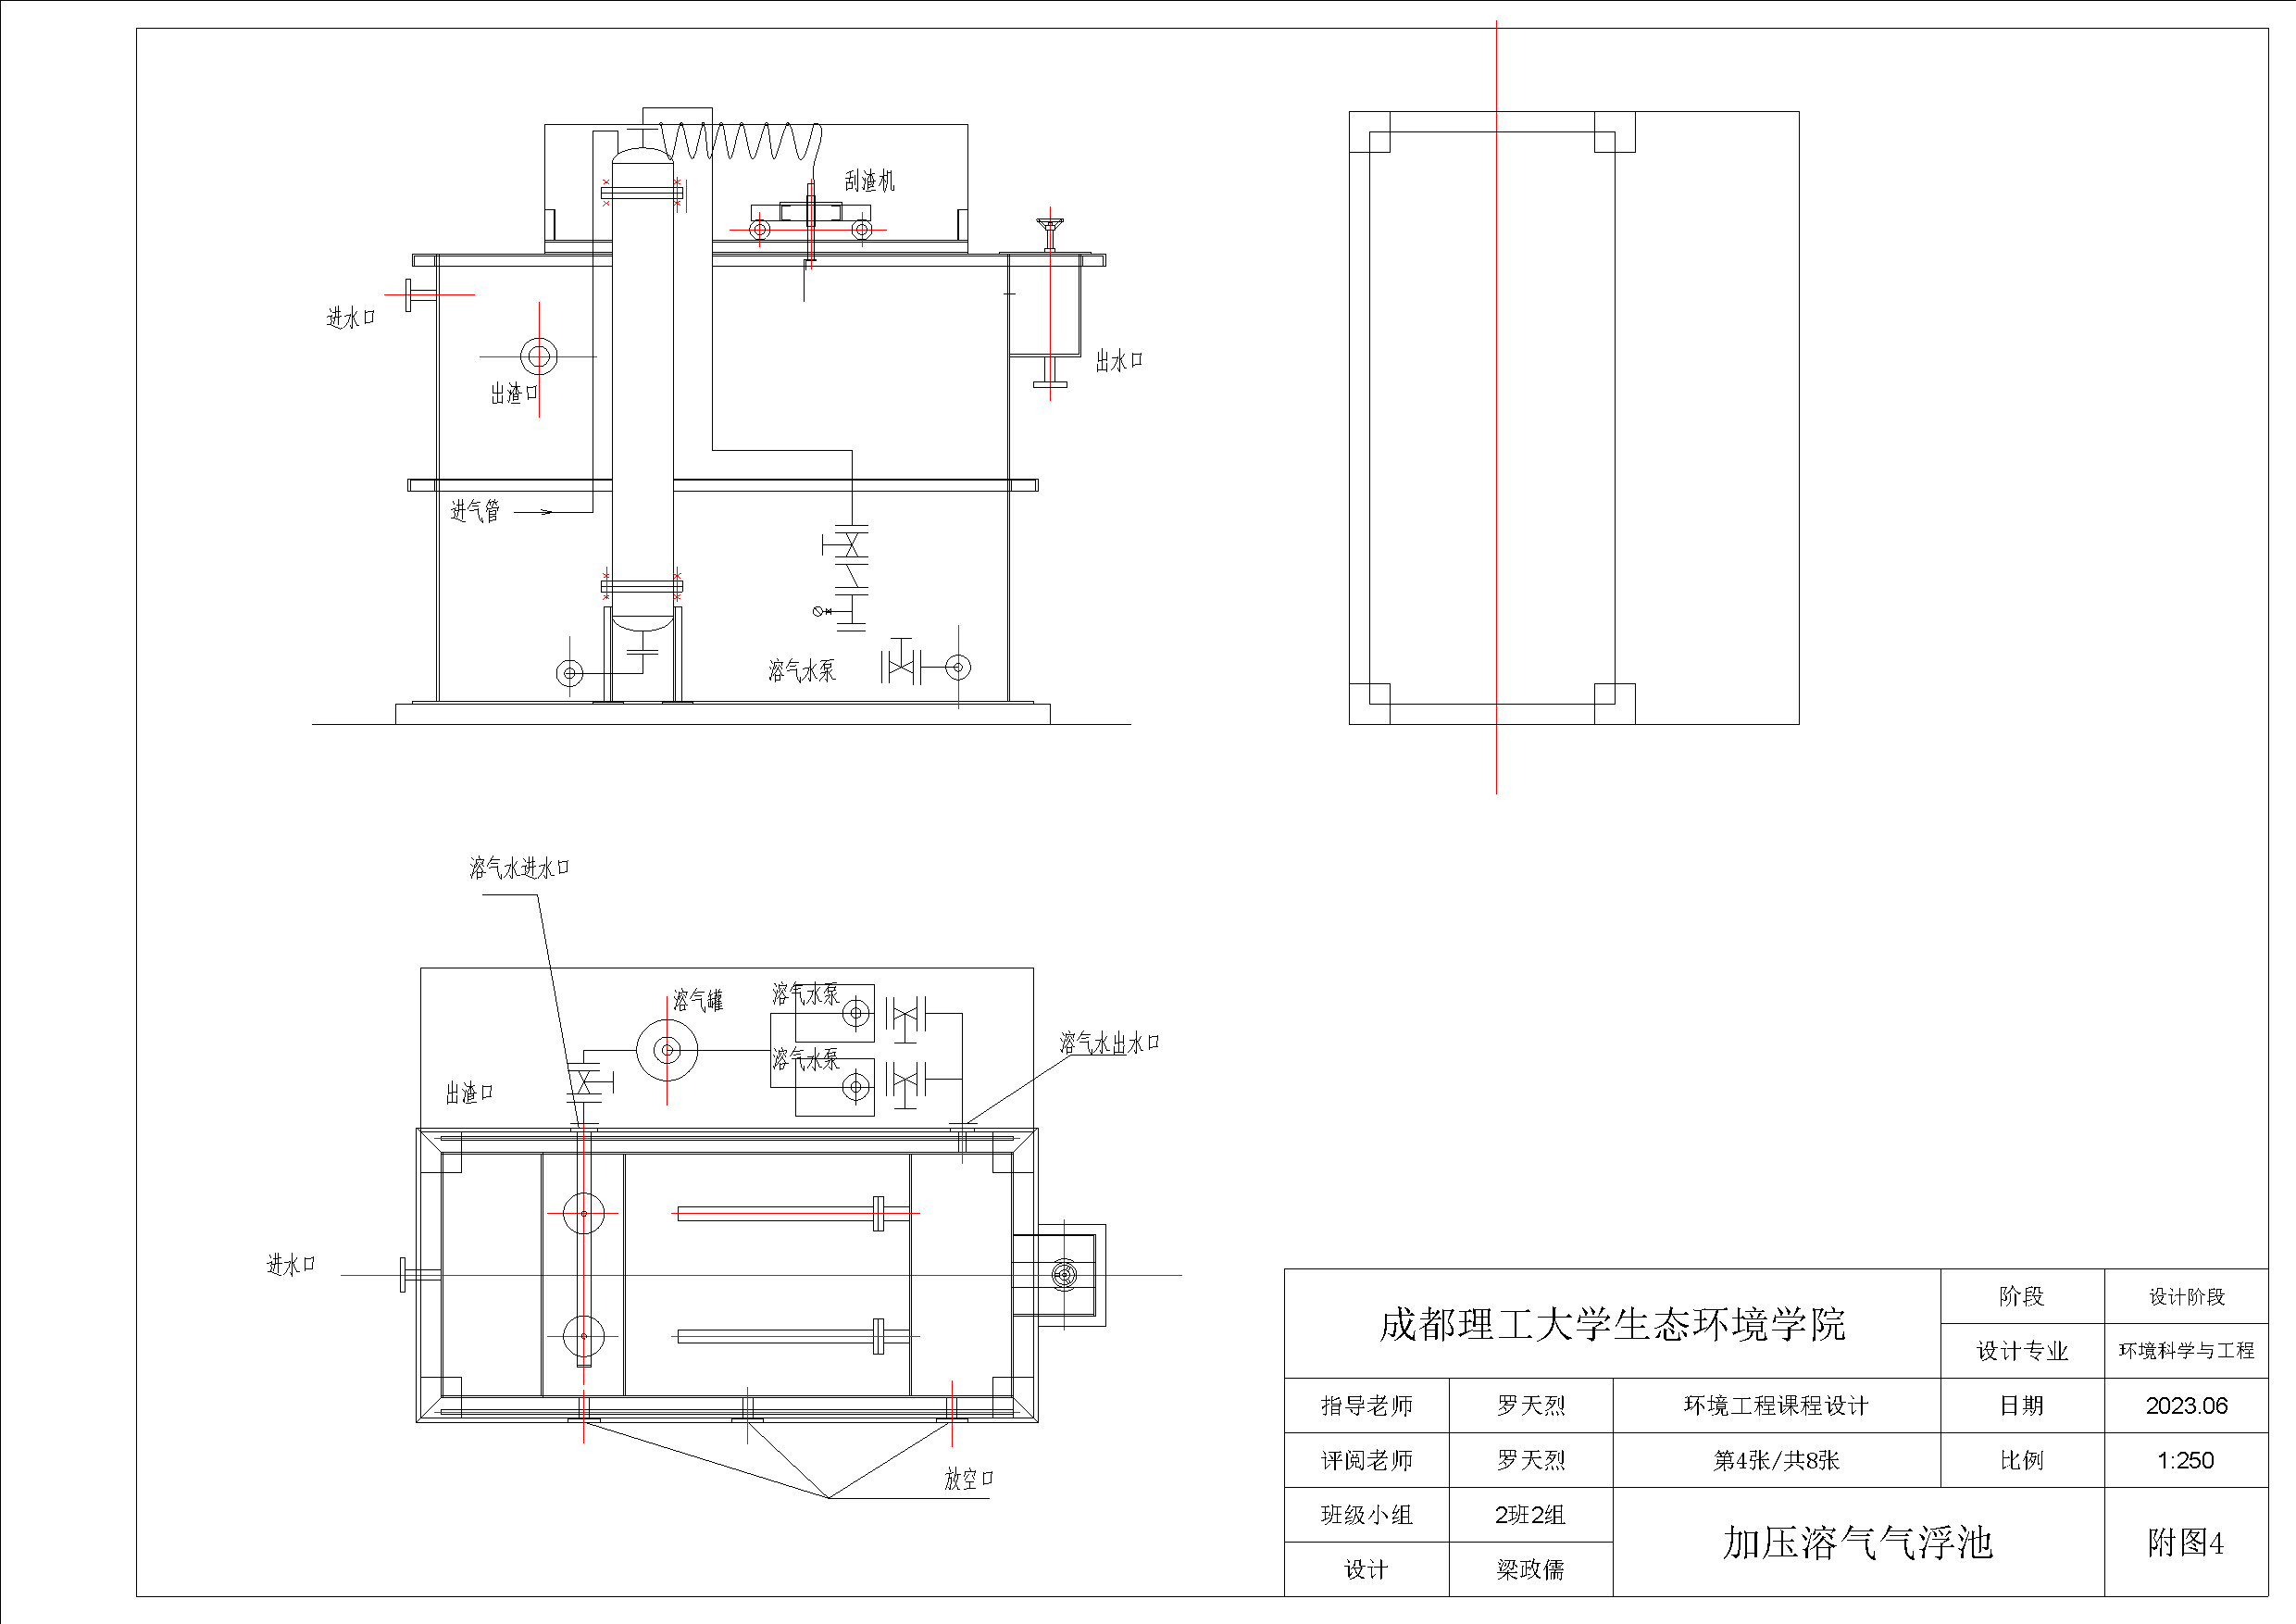
\includegraphics[width=1.15\textwidth]{drawing/Flat section of a pressurized air flotation tank.pdf}}
\end{figure}

\thumbnail{臭氧消毒池平剖面图}
\begin{figure}[H]
	\centering
	\rotatebox{90}{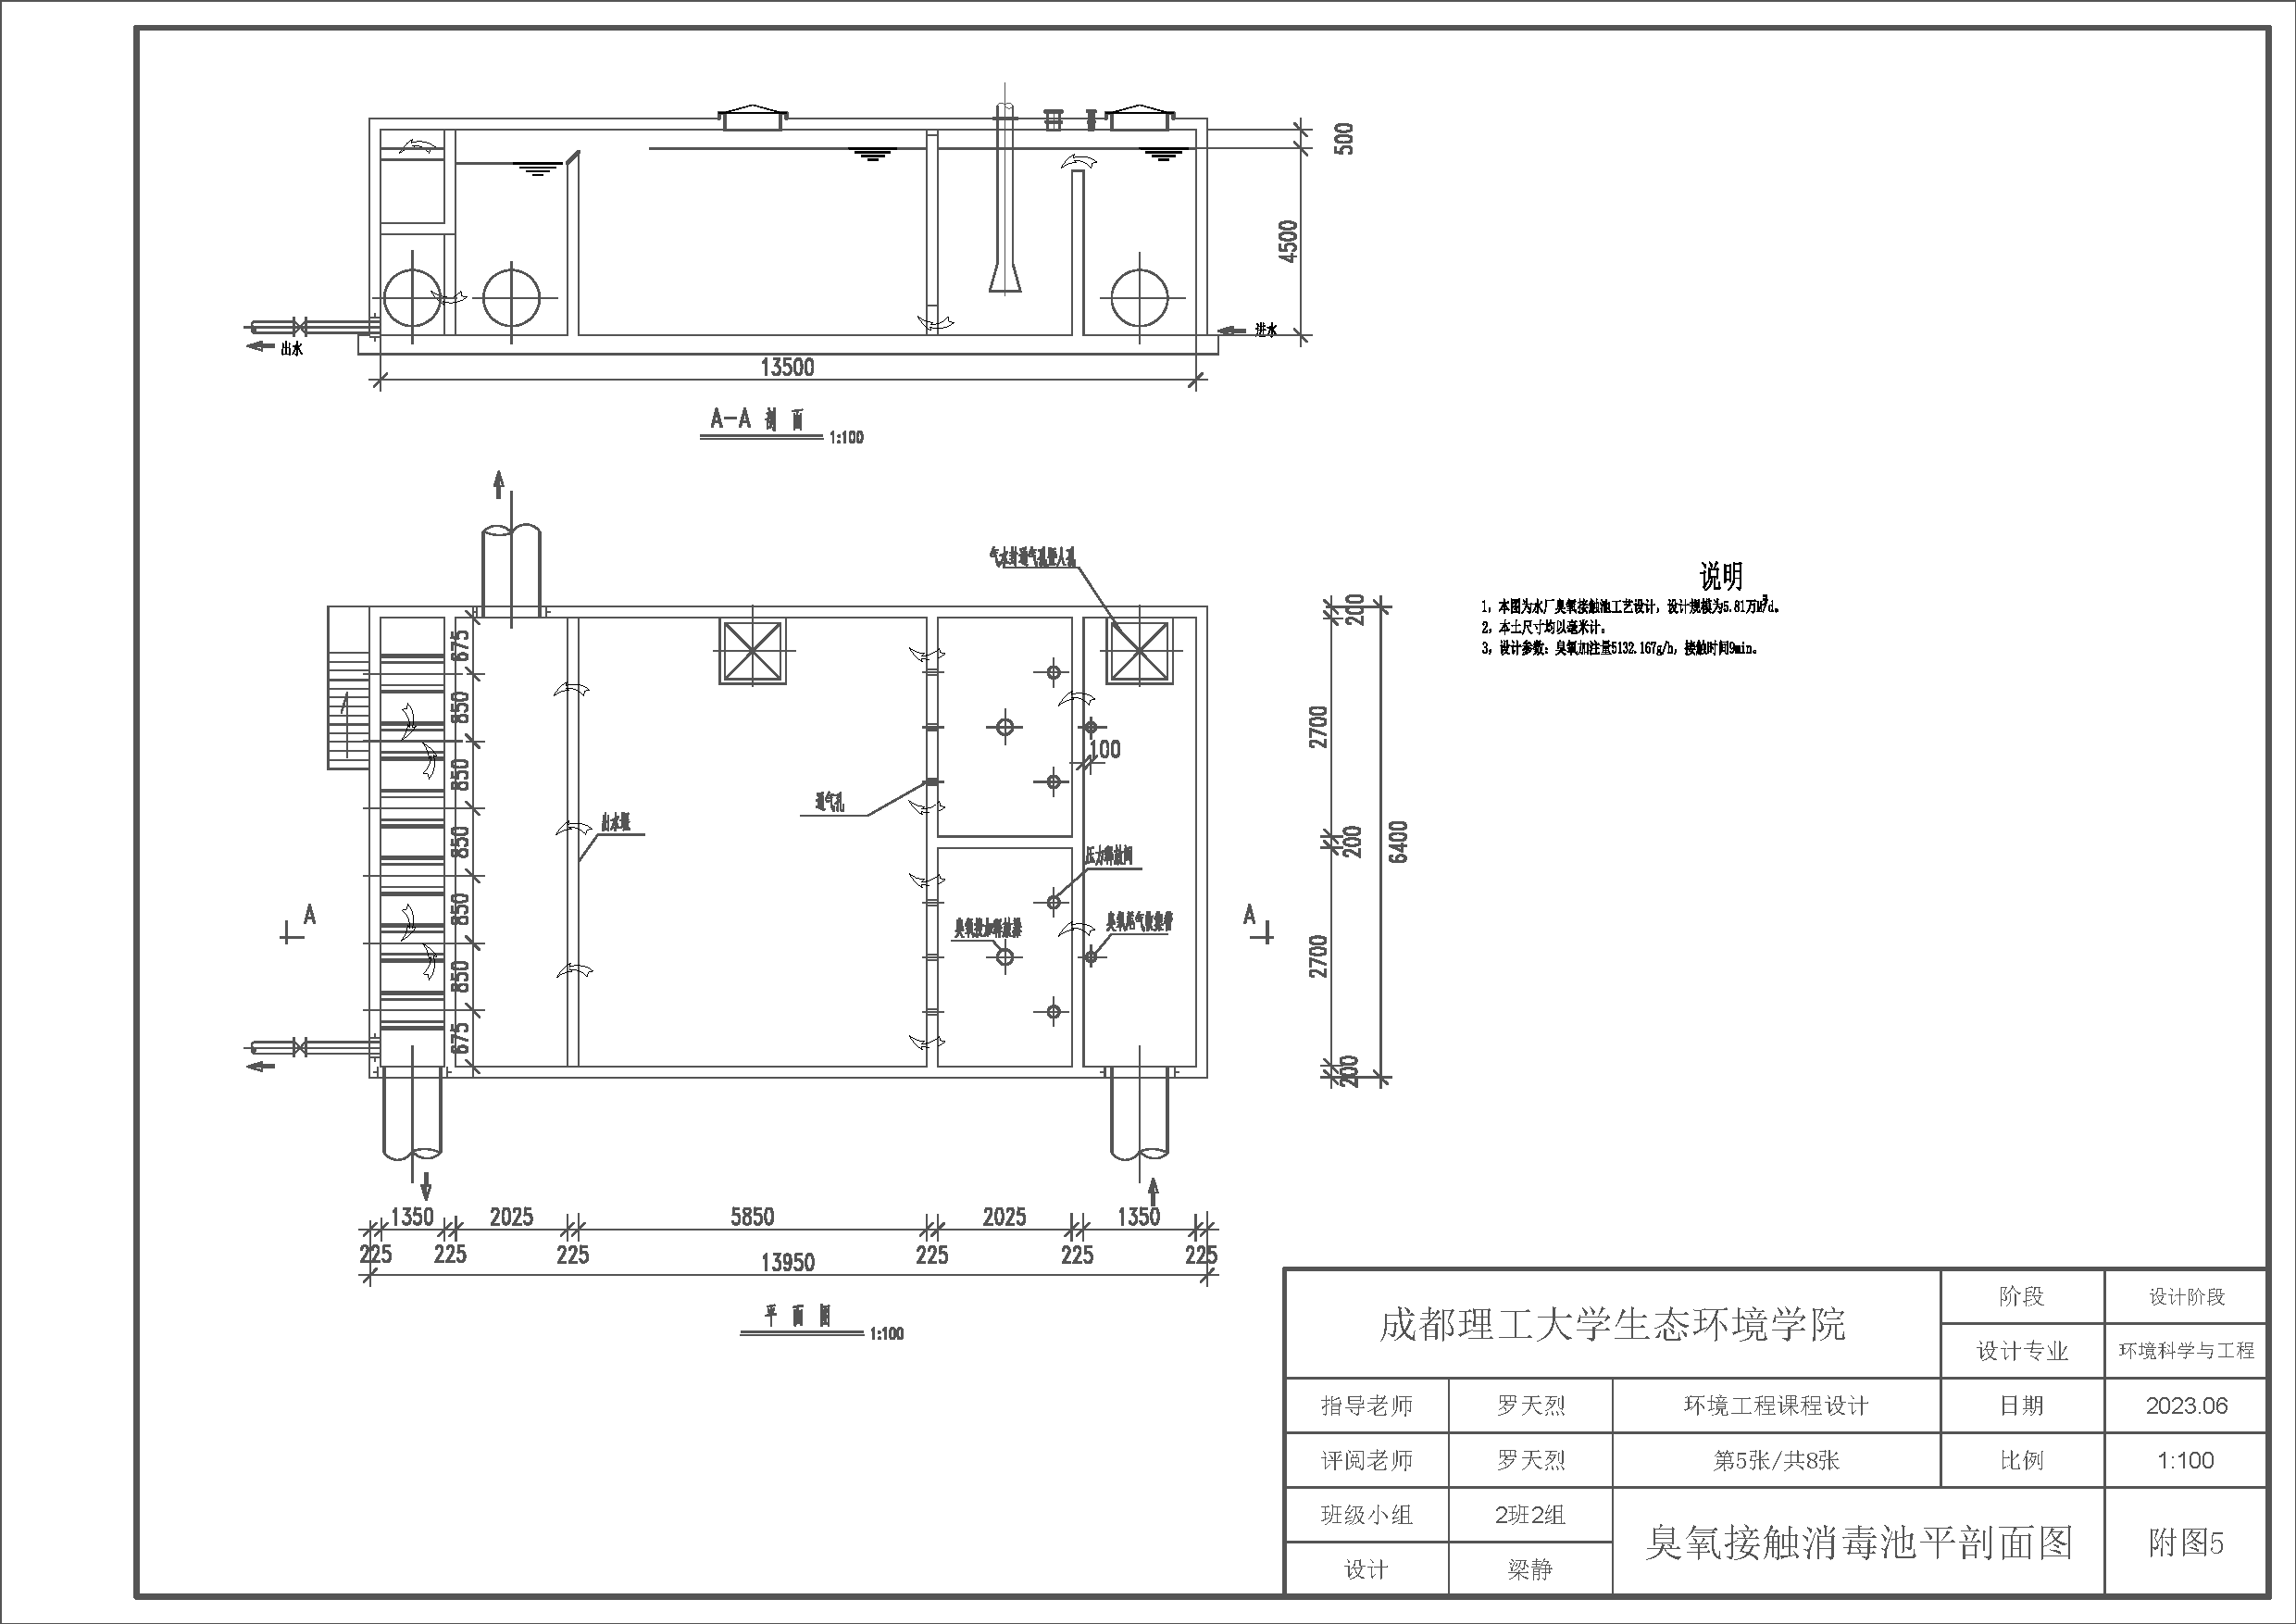
\includegraphics[width=1.15\textwidth]{drawing/Flat profile view of ozone disinfection tank.pdf}}
\end{figure}

\thumbnail{提升泵房平剖面图}
\begin{figure}[H]
	\centering
	\rotatebox{90}{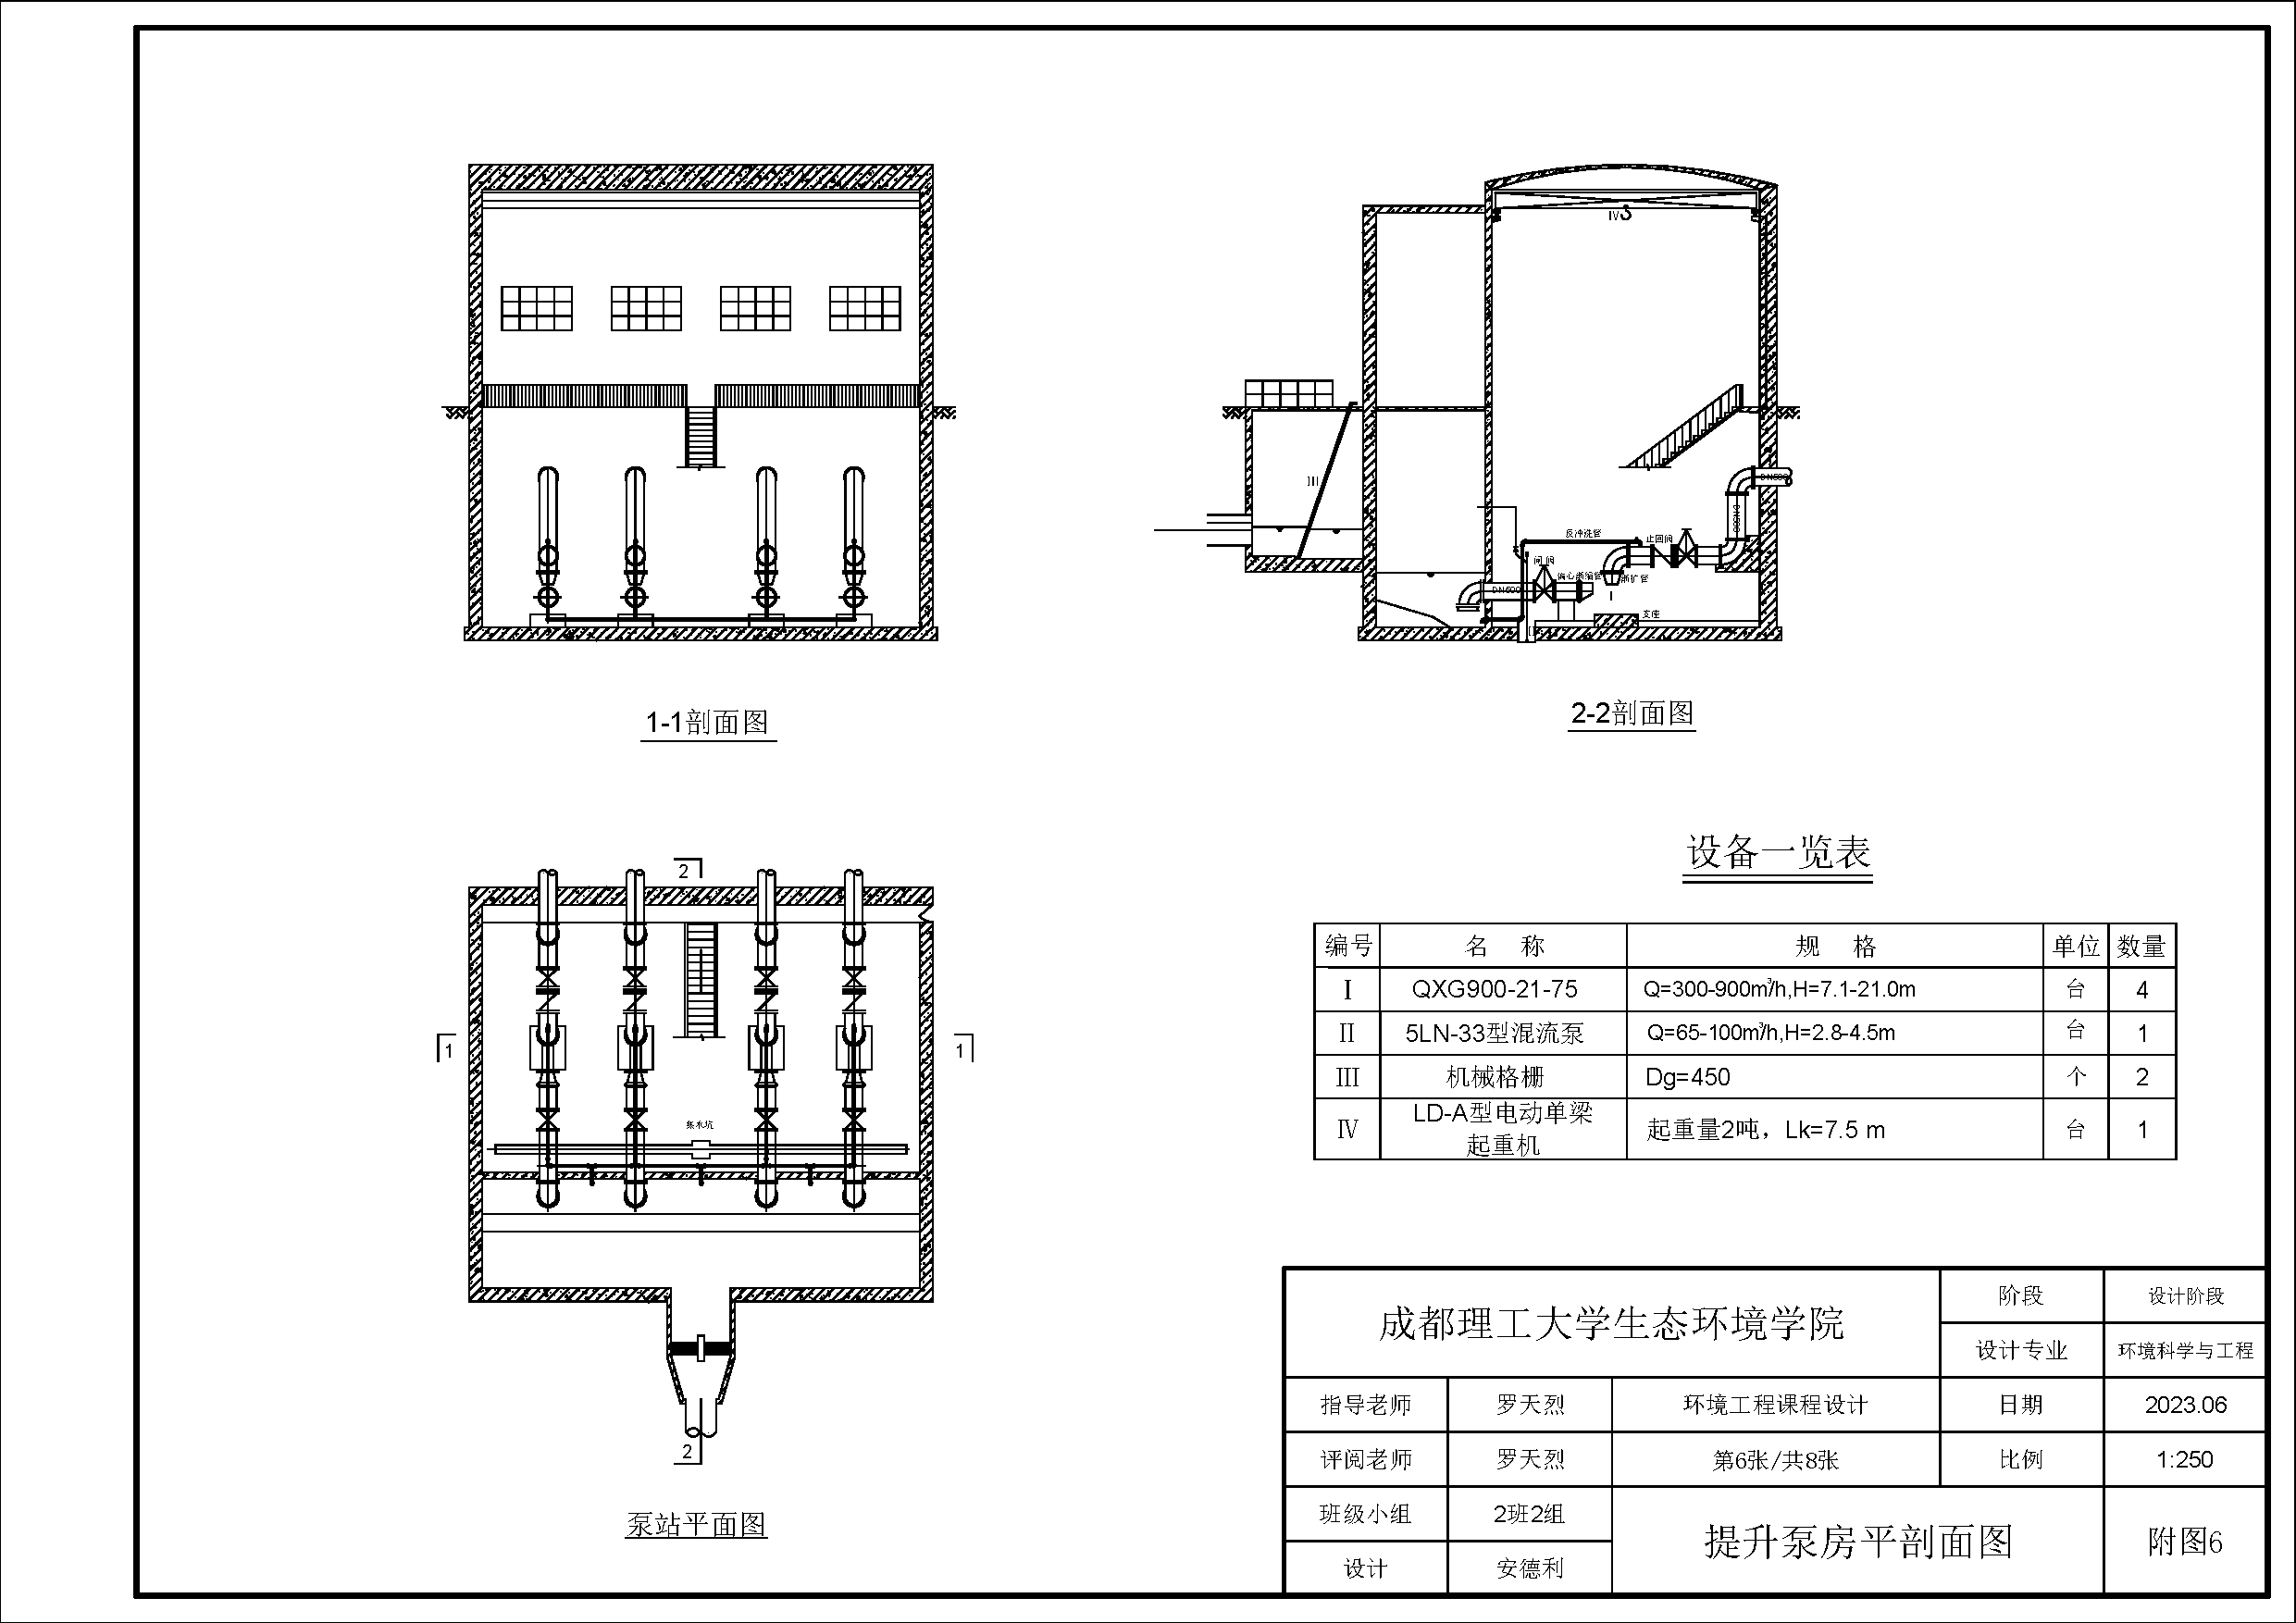
\includegraphics[width=1.15\textwidth]{drawing/Flat profile view of the lifting pump room.pdf}}
\end{figure}

\thumbnail{污水处理厂平面布置图}
\begin{figure}[H]
	\centering
	\rotatebox{90}{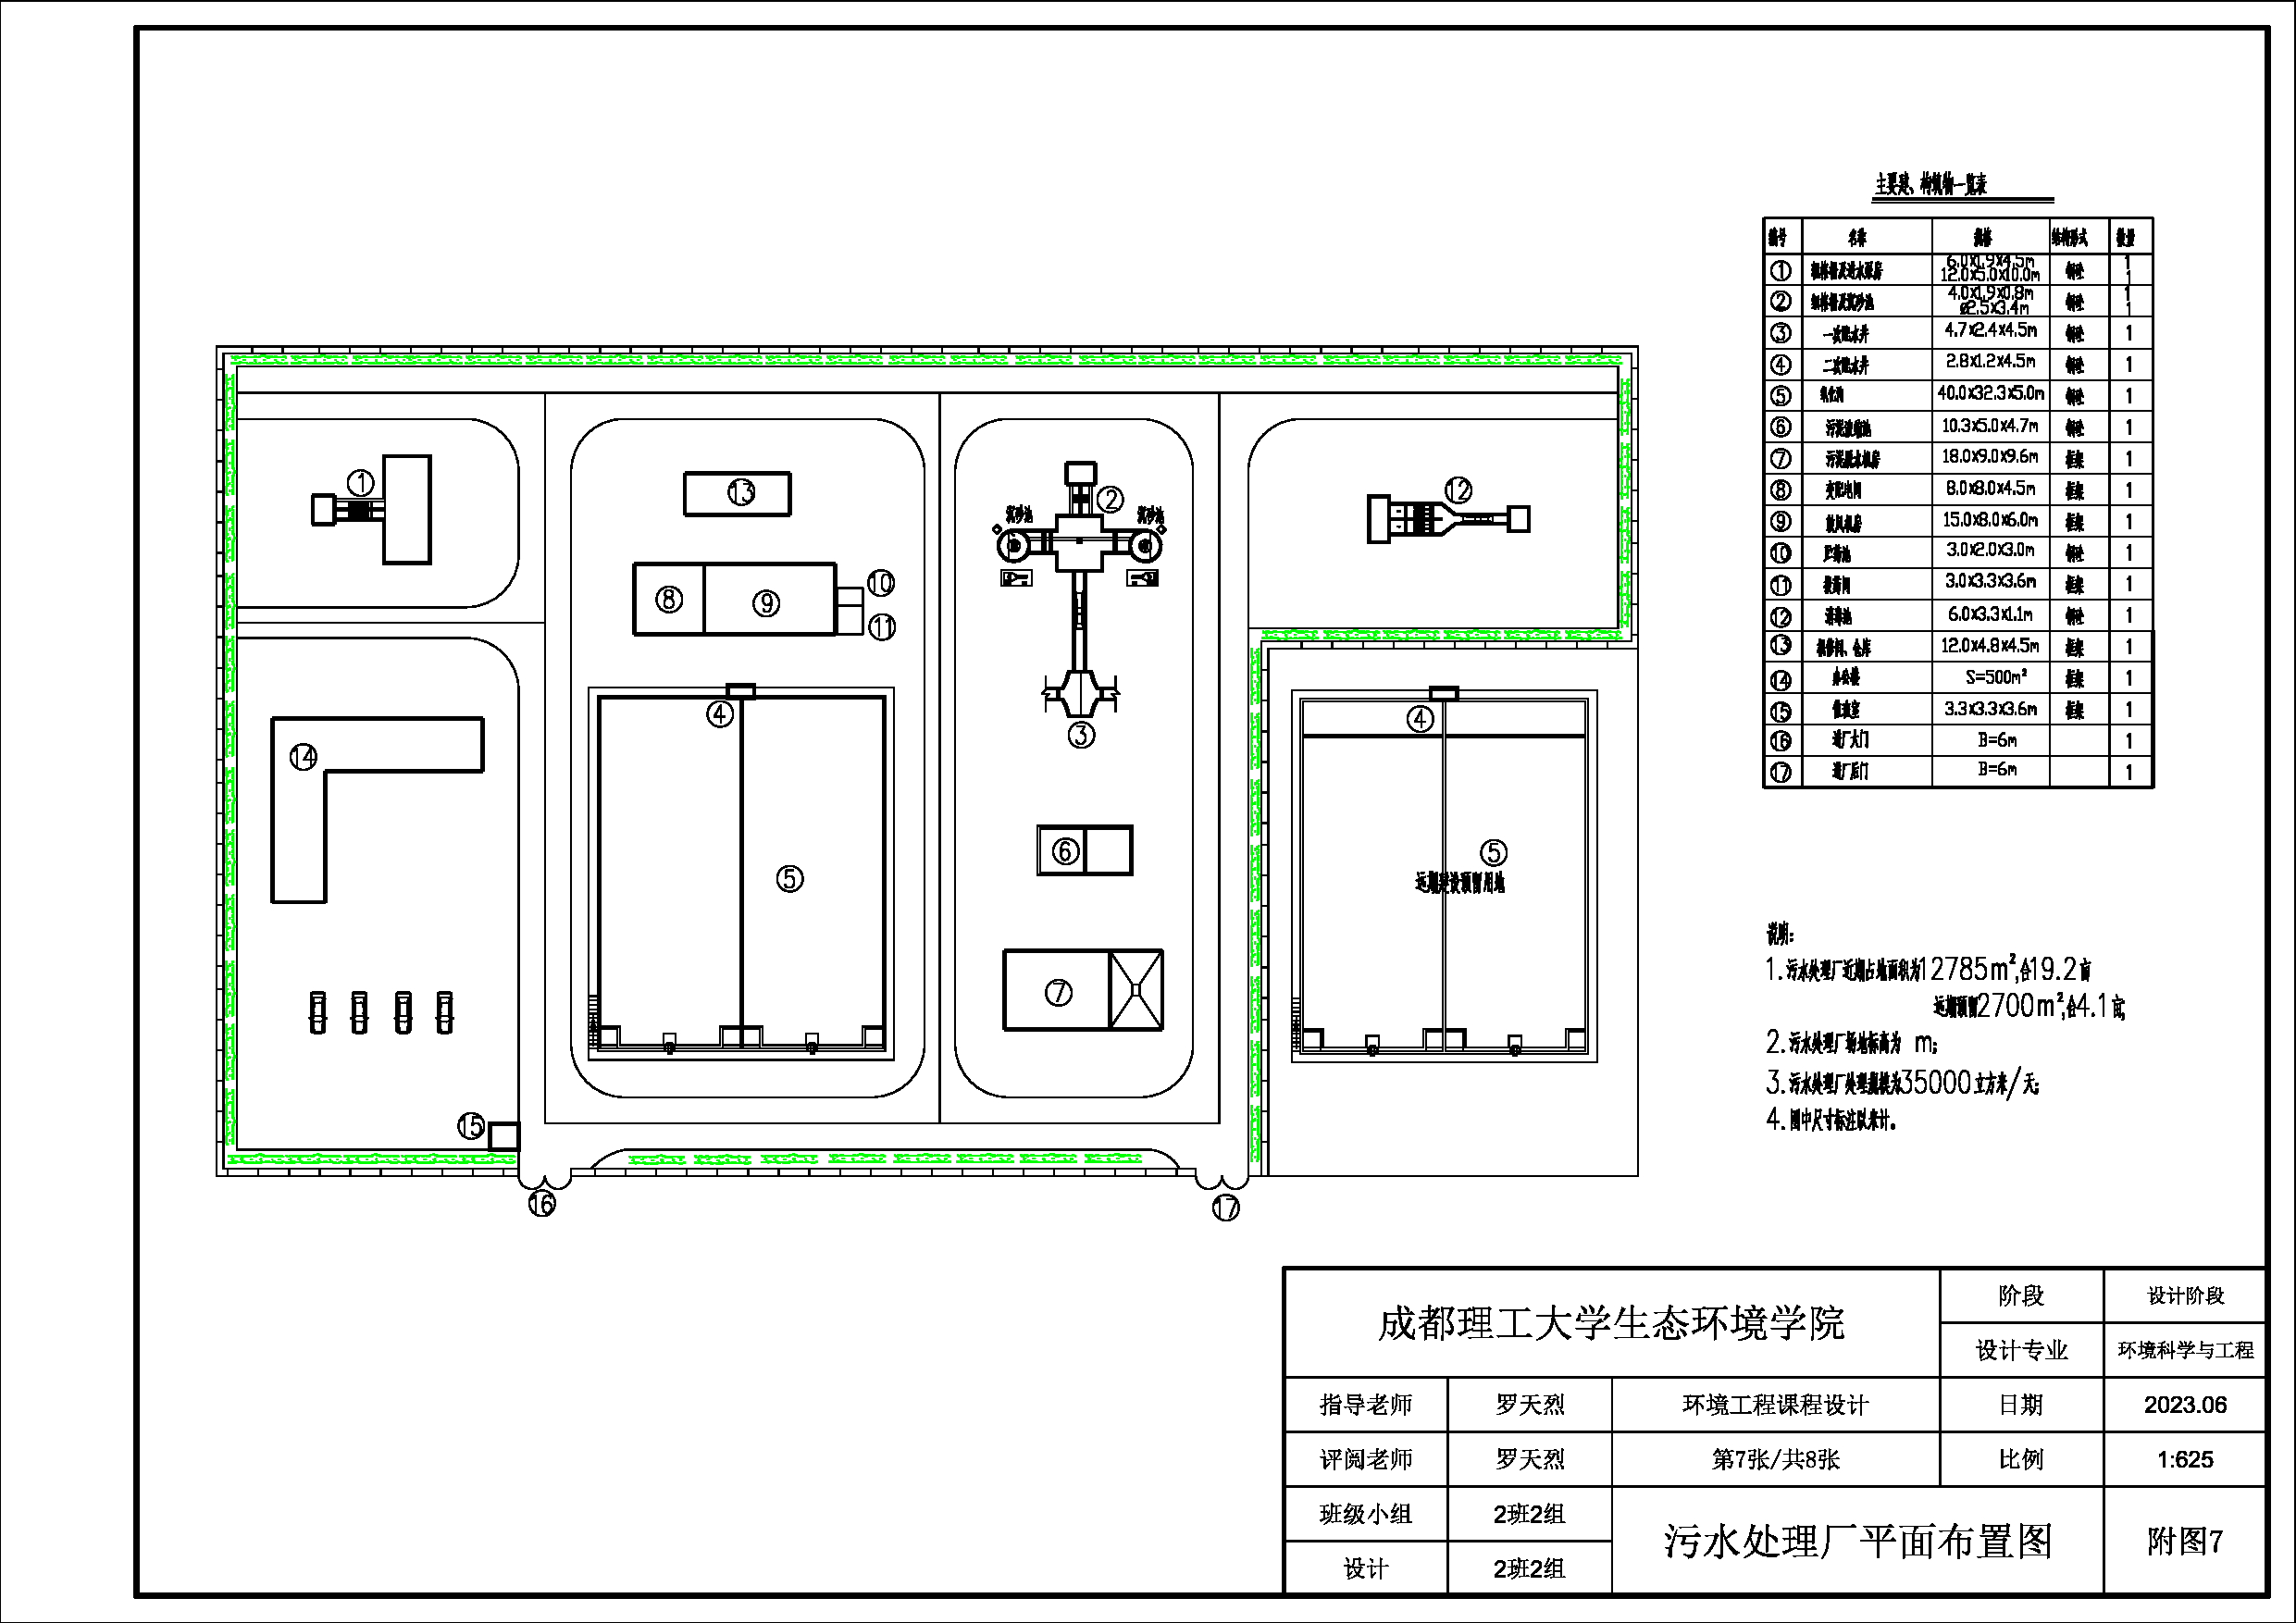
\includegraphics[width=1.15\textwidth]{drawing/Floor plan of the sewage treatment plant.pdf}}
\end{figure}

\thumbnail{污水处理厂高程布置图}
\begin{figure}[H]
	\centering
	\rotatebox{90}{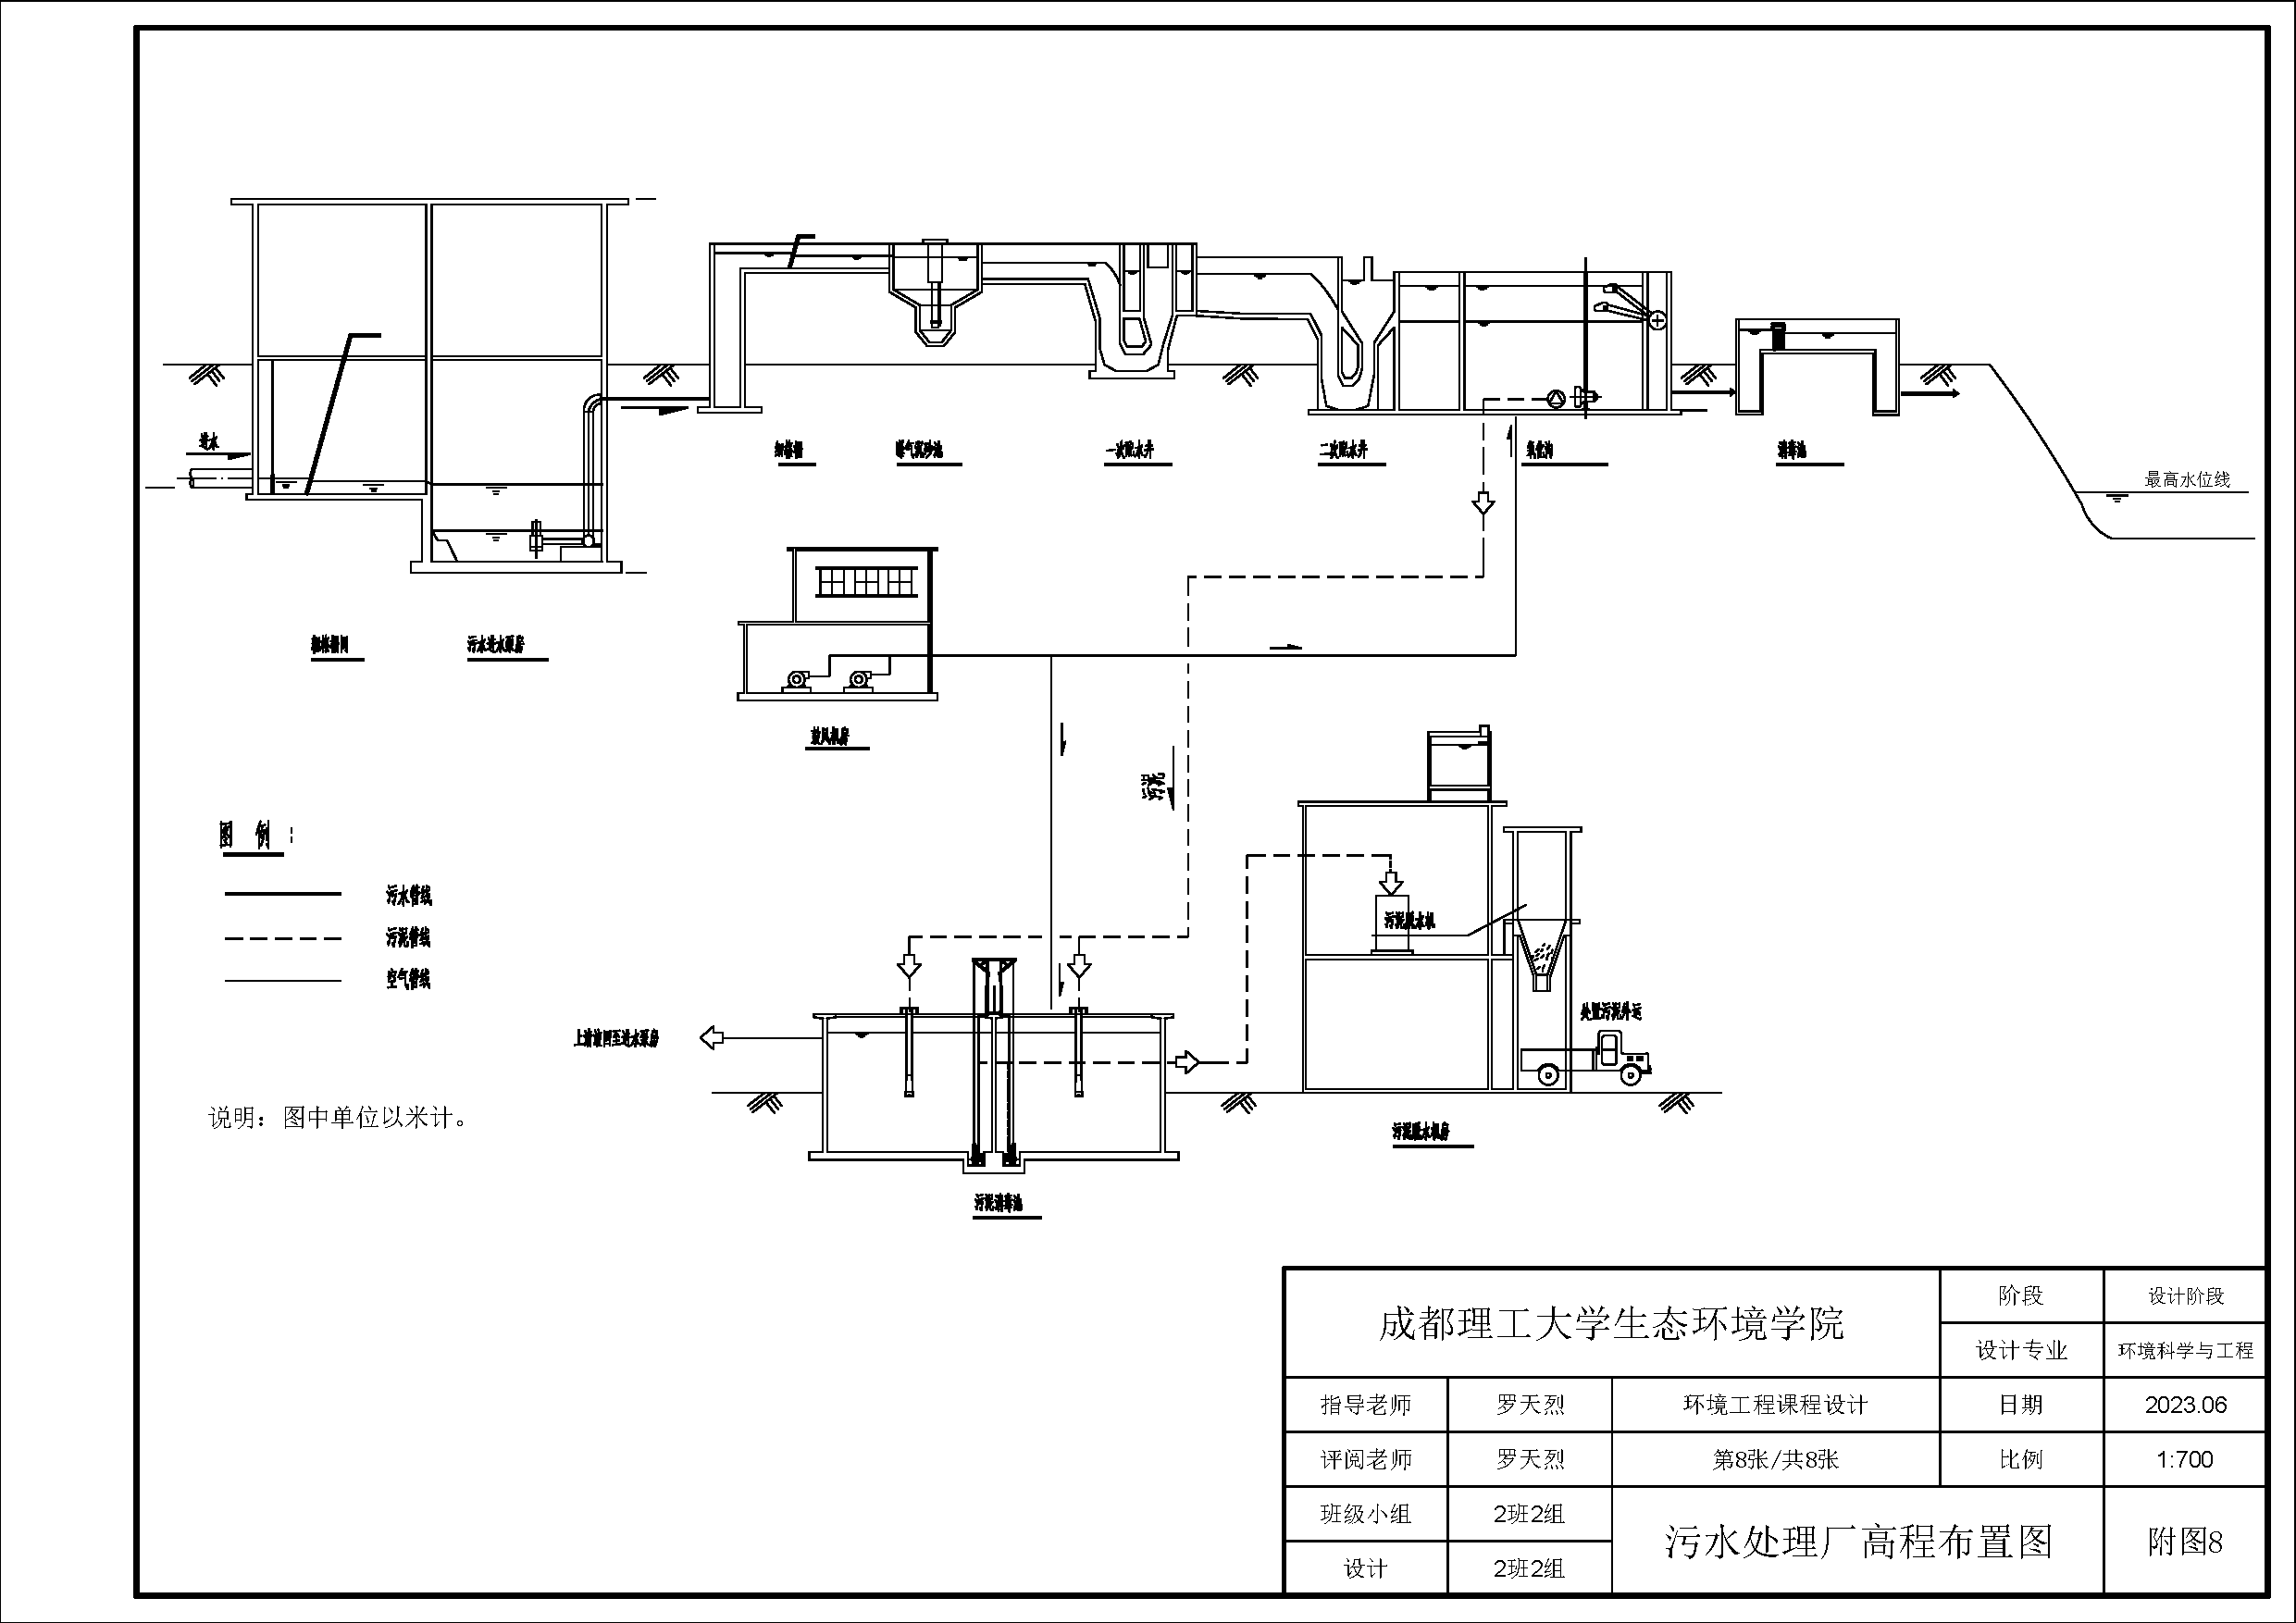
\includegraphics[width=1.15\textwidth]{drawing/Elevation layout of a sewage treatment plant.pdf}}
\end{figure}

